\chapter{User Guide}
\section{Instructions}
You must provide an adequate user guide for your software. The guide should provide easily understood instructions on how to use your software. A particularly useful approach is to treat the user guide as a walk-through of a typical session, or set of sessions, which collectively display all of the features of your package. Technical details of how the package works are rarely required. Keep the guide concise and simple. The extensive use of diagrams, illustrating the package in action, can often be particularly helpful. The user guide is sometimes included as a chapter in the main body of the report, but is often better included in an appendix to the main report.
-how to set up (commands)//d
-how to use given pieces of sample text//d
-images//d

\par For the zipped file given, unzip them. In the unzip folder there is a build.gradle file which can be used by used by Gradle locally (if it installed), and by the Gradle wrapper provided in the zip. It is advised to install Gradle\footnote{\url{https://gradle.org/install}}, specifically the latest version (v3.4.1+). See Figure \ref{fig:gradleVersion}.

\begin{figure}[H]
\caption{Command to see the version of Gradle Installed. Will only work if Gradle is installed.}
\label{fig:gradleVersion}
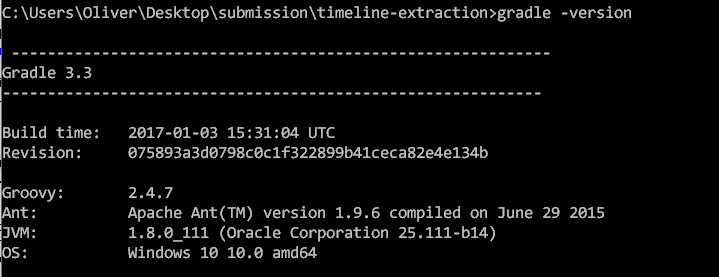
\includegraphics{gradleVersion.PNG}
\centering
\end{figure}


\par To run the system traverse to the root directory of the unzipped folder (see Figure \ref{fig:folderDirectory}) in command-line or terminal (see Figure \ref{fig:traverseToRootDir}). If Gradle is locally installed, to build the system (i.e. retrieve the libraries, and run the tests) use the command: \textbf{gradle build} (see Figure \ref{fig:gradleBuild}). To run the actual application with the interacting UI to load documents, use the command: \textbf{gradle run} (see Figure \ref{fig:gradleRun}). To run the 35 unit tests, to ensure the application is functioning correctly, use the command: \textbf{gradle test} (see Figure \ref{fig:gradleTest}). The unit tests include tests on file processing, JSON converting, and event creation.

\begin{figure}[H]
\caption{Unzipped Folder contents}
\label{fig:folderDirectory}
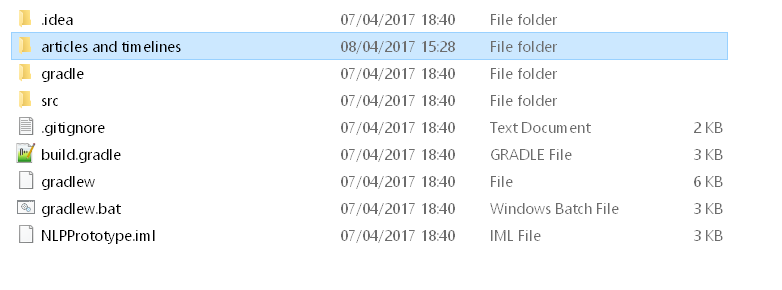
\includegraphics{folderDirectory.PNG}
\centering
\end{figure}

\begin{figure}[H]
\caption{Traversing to Root directory of project in command line.}
\label{fig:traverseToRootDir}
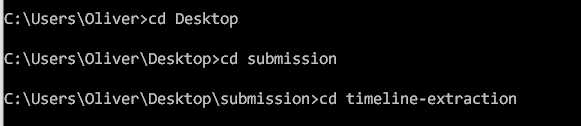
\includegraphics{traverseToRootDir.PNG}
\centering
\end{figure}

\begin{figure}[H]
\caption{Effects of running the command: gradle run}
\label{fig:gradleRun}
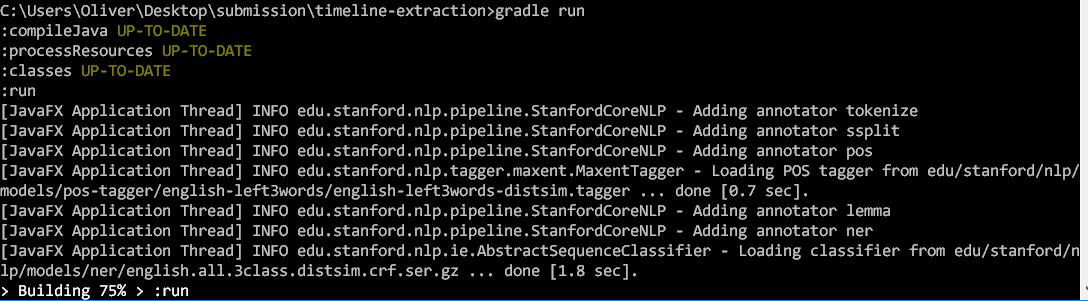
\includegraphics[width=\linewidth]{gradleRun.PNG}
\centering
\end{figure}

\begin{figure}[H]
\caption{Effects of running the command: gradle build.}
\label{fig:gradleBuild}
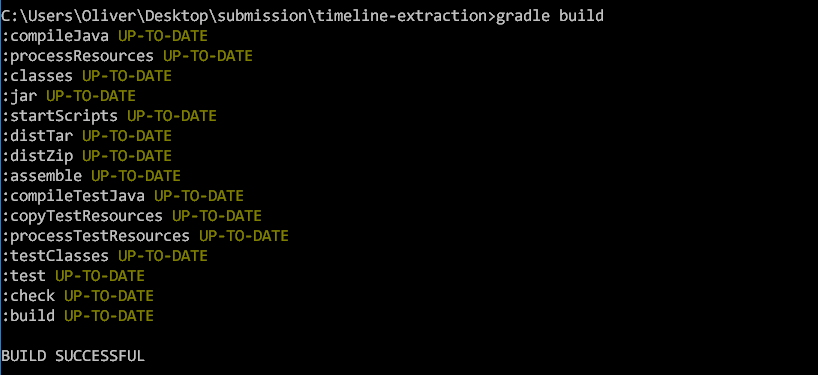
\includegraphics[width=\linewidth]{gradleBuild.PNG}
\centering
\end{figure}

\begin{figure}[H]
\caption{Effects of running the command: gradle test}
\label{fig:gradleTest}
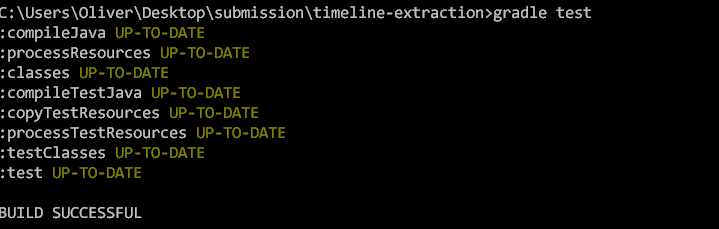
\includegraphics{gradleTest.PNG}
\centering
\end{figure}

\par If Gradle is not installed, the Gradle wrapper can be used. First, in command line, traverse the system's file space to the root directory of the project. In the root directory, to build the system use the command: \textbf{gradlew build} (see Figure \ref{fig:gradlewBuild}). To run the actual application, use the command: \textbf{gradlew run} (see Figure \ref{fig:gradlewRun}). To run the tests, use the command: \textbf{gradlew test} (see Figure \ref{fig:gradlewTest}).

\begin{figure}[H]
\caption{Effects of running the command: gradlew run}
\label{fig:gradlewRun}
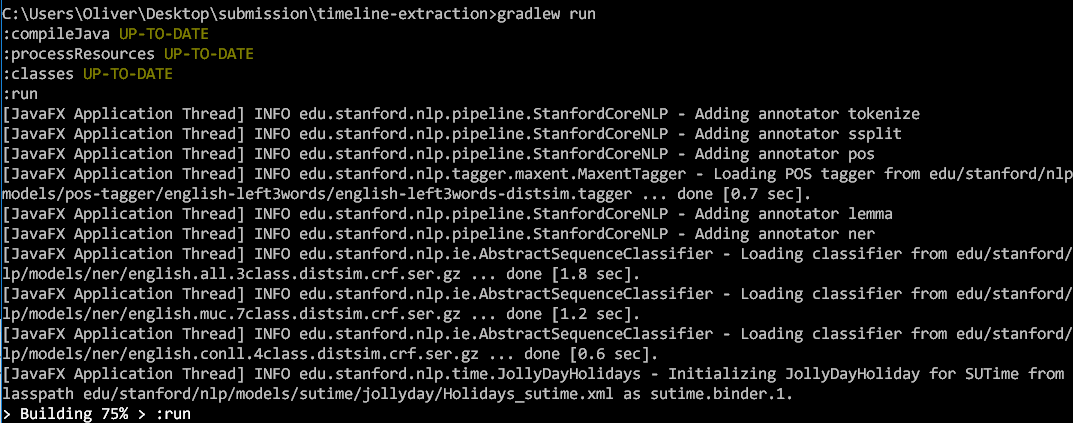
\includegraphics[width=\linewidth]{gradlewRun.PNG}
\centering
\end{figure}

\begin{figure}[H]
\caption{Effects of running the command: gradlew build}
\label{fig:gradlewBuild}
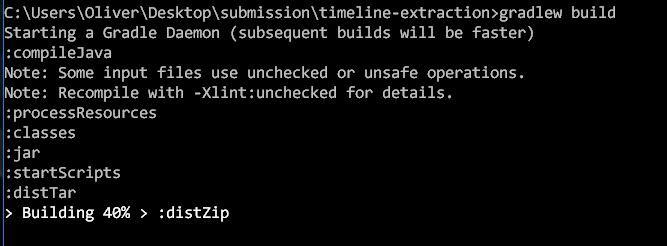
\includegraphics{downloadingLibraries.PNG}
\centering
\end{figure}

\begin{figure}[H]
\caption{Effects of running the command: gradlew test}
\label{fig:gradlewTest}
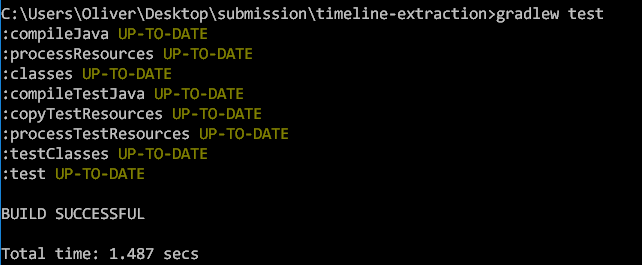
\includegraphics{gradlewTest.PNG}
\centering
\end{figure}

\par Once the system is running, a GUI is shown inviting the user to load documents. Pressing on the button will open the file chooser dialog to choose PDF, TXT, or DOCX files to load (see Figures \ref{fig:fileDirectory} and \ref{fig:confirmArticles}). The sample documents provided in the submission can be used. Once these have been loaded a timeline will be shown. Initially, the traditional timeline is shown (see Figure \ref{fig:loaded}), to swap to the Range Timeline use the Timeline menu option to select it. An event can be edited by pressing on the `Edit Event' button, where a dialog is shown to edit its data (see Figure \ref{fig:editEvent}). If the data is not valid, the user will be informed by highlighting in red the input field that is invalid. When no data is present, a hint is given for the input format (e.g. for dates the input format is: dd-MM-yyyy, where dd is a day value from 01 to 31m MM a month value from 01 to 12, and yyyy a year value from 0001 to 9999). Events can be deleted from the timeline through the `Delete' button in the `Edit Event' dialog. More documents can be loaded using the `Load Documents' button. Events relating to a document can be removed by pressing on the red cross next to a document in the `Document Viewer' (see Figure \ref{fig:removeDoc}). To view the sentence that produced an event, use the `View' button from an event.

\begin{figure}[H]
\caption{Confirming the reference points/base dates used for the articles when they are being processed.}
\label{fig:confirmArticles}
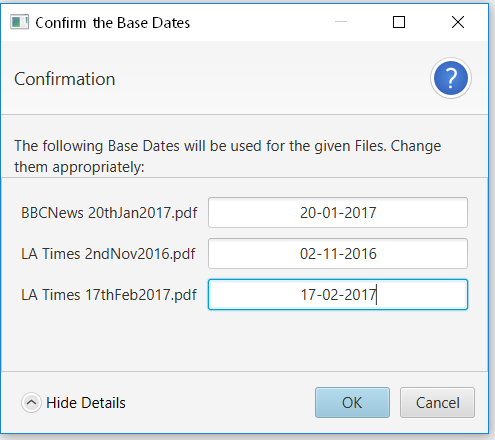
\includegraphics{confirmArticles.PNG}
\centering
\end{figure}

\begin{figure}[H]
\caption{Window shown when the documents have been processed.}
\label{fig:loaded}
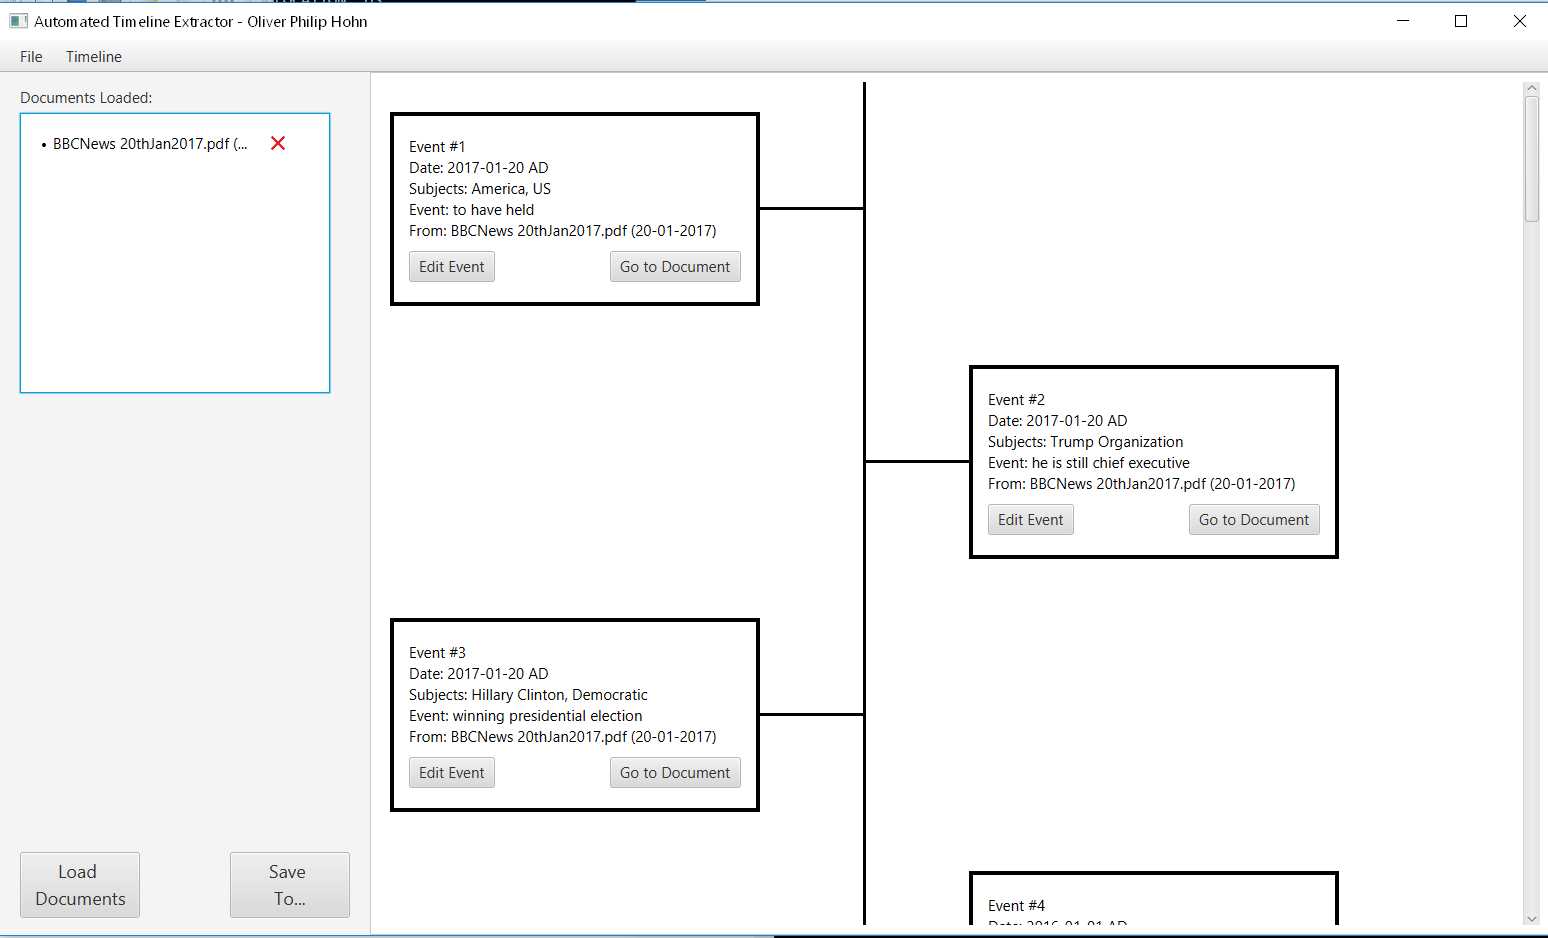
\includegraphics[width=\linewidth]{loaded.PNG}
\centering
\end{figure}


\begin{figure}[H]
\caption{Dialog to edit an event.}
\label{fig:editEvent}
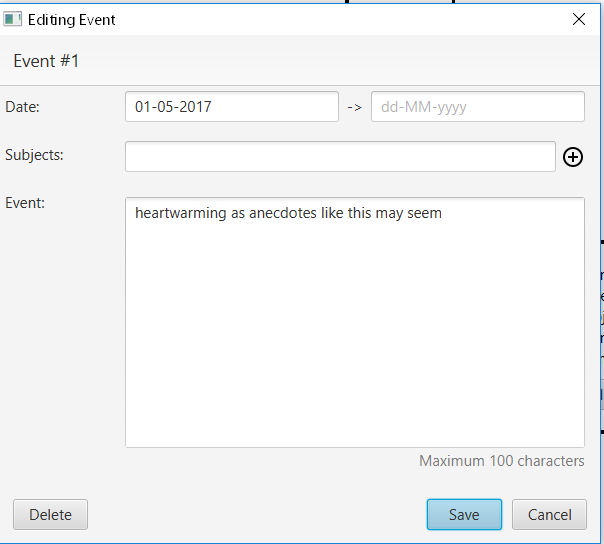
\includegraphics{editEvent.PNG}
\centering
\end{figure}

\begin{figure}[H]
\caption{Row of a document, with the red cross to remove its events from the timeline.}
\label{fig:removeDoc}

\includegraphics{removeDoc.PNG}
\centering
\end{figure}

\par Settings can be changed using the File->Preferences... menu item (see Figure \ref{fig:preferences}). This allows the user to change document processing such as how many threads used, and the threshold value used for summaries, as well as GUI settings such as start up width and height of the window. Saving the Settings will produce a System.ini file in the root directory.

\begin{figure}[H]
\caption{Dialog to view/edit the preferences of the system.}
\label{fig:preferences}
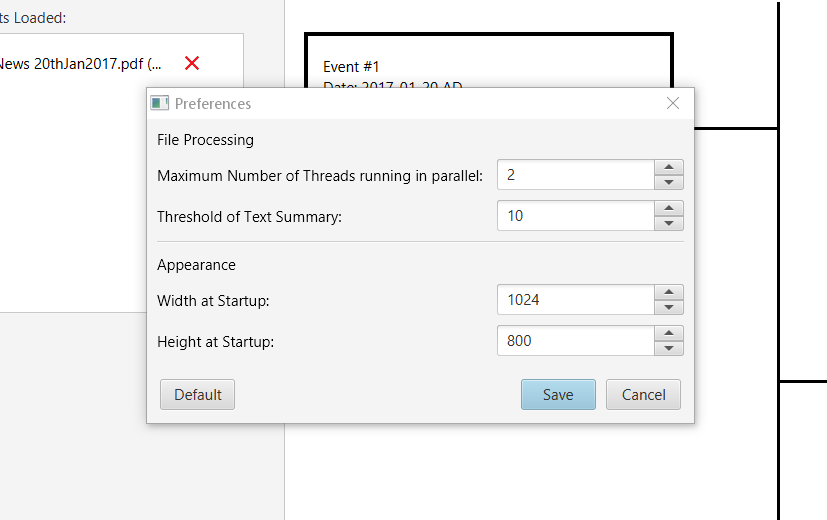
\includegraphics{preferences.PNG}
\centering
\end{figure}

\par To save a timeline, the `Save To..' button can be used (see Figure \ref{fig:saveTo}). This allows the user to decide the file format to save the timeline to, JSON or PDF. Afterwhich the file chooser dialog is shown to choose the location to save the timeline file. If it cannot be saved at that location, the user will be notified, and asked to select a new location.

\begin{figure}[H]
\caption{Dialog asking the user to choose their file format to save the timeline, after this a File Chooser is shown for the user to select the location to save the timeline in.}
\label{fig:saveTo}
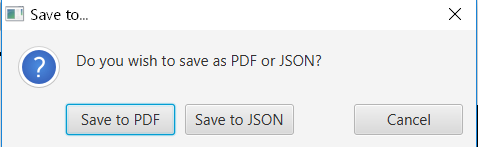
\includegraphics{saveTo.PNG}
\centering
\end{figure}